%\documentclass[11pt]{article} %指定文档的类型和基本格式。这里选择了article类,字体大小为11磅。
\documentclass[UTF8]{ctexart}
\usepackage{amsmath,textcomp,amssymb,geometry,graphicx,enumerate} %加载了一些宏包,这些宏包提供了额外的功能和格式设定,例如数学符号、文本特殊符号、排版布局等。

\usepackage{listings}
\usepackage[dvipsnames]{xcolor}
\usepackage{mdframed}

%\usepackage[utf8]{inputenc}
%\usepackage{xeCJK} % Added for Chinese support
%\setCJKmainfont{SimSum} % Set the Chinese font, you can change it to any font you have


%\def\Name{zilong}
\def\Name{王子隆}  % Your name 定义了一个名为\Name的变量,它的内容是"PUT SOMETHING HERE"。通常这个变量会在文档中被调用以插入相应的信息。
\def\SID{2221411126}  % Your student ID number 定义了一个名为\SID的变量,它的内容也是"PUT SOMETHING HERE"。
\def\Lab{1} % Number of Lab 定义了一个名为\Lab的变量,它的内容是"n",表示编号。
\def\Session{Autumn 2023} %定义了一个名为\Session的变量,它的内容是"Autumn 2023",表示学期。
\def\Class{计算机2204}

\title{DS--Autumn 2023 --- Laboratory report} %设置了文档的标题,包括课程名、学期和作业编号。
\author{\Name, 学号 \SID, 班级 \Class} %设置了文档的作者信息,使用了之前定义的\Name和\SID变量。
\markboth{DS--\Session\  Lab  \Name}{DS--\Session\ Lab  \Name} %设置了页眉的内容。
\pagestyle{myheadings} %设置了页眉的内容。
\date{\today} %清空了默认的日期显示。

\newenvironment{qparts}{\begin{enumerate}[{(}a{)}]}{\end{enumerate}} %定义了一个新的环境qparts,用于创建带有小括号标记的题目部分。
%\def\endSolutionsmark{$\mathcal{X} \mathcal{I} \mathcal{U} $} %定义了证明结束标记为一个方框符号。
\newenvironment{Solutions}{\par{\bf Solutions}:}%{\endSolutionsmark\smallskip} %定义了一个新的环境Solutions,用于书写数学证明。


\lstdefinestyle{javastyle}{ %%定义了一个样式mystyle,指定了Java语言,设定了代码的基本样式、注释样式、关键词样式等等
    language=Java,
    basicstyle=\ttfamily\small, % 设置代码字体为大一些
    commentstyle=\color{OliveGreen},
    keywordstyle=\color{RoyalBlue},
    numberstyle=\tiny\color{gray},
    numbers=left,
    frame=single,
    breaklines=true,
    breakatwhitespace=true,
    tabsize=4
}

\lstdefinestyle{cppstyle}{
    language=C++,
    basicstyle=\ttfamily\small,
    commentstyle=\color{OliveGreen},
    keywordstyle=\color{RoyalBlue},
    numberstyle=\tiny\color{gray},
    numbers=left,
    frame=single,
    breaklines=true,
    breakatwhitespace=true,
    tabsize=4
}
\definecolor{lightgray}{RGB}{240,240,240}  % 自定义淡灰色

\newmdenv[linecolor=black,linewidth=1pt,backgroundcolor=lightgray]{exampleframe}

\textheight=9in
\textwidth=6.5in
\topmargin=-.75in
\oddsidemargin=0.25in
\evensidemargin=0.25in %设置了页面的尺寸和边距。



\begin{document}
\maketitle

%Collaborators: PUT SOMETHING HERE (LIST OF YOUR COLLABORATORS, OR WRITE NONE)

\section*{lab1. 背包问题}
\subsection*{题目}
\begin{abstract}
    %Abstract goes here...
    \textbf{1.问题描述}


    假设有一个能装入总体积为T的背包和n件体积分别为$w_1,w_2,$…$w_n$的物品,能否从n件物品中挑选若干件恰好装满背包,
    即使$w_1+w_2+$…$+w_m=T$,要求找出所有满足上述条件的解。 
   
    例如:当$T=10$,各件物品的体积{1,8,4,3,5,2}时,可找到下列4组解:

    (1,4,3,2)     (1,4,5)     (8,2)     (3,5,2)。

    \textbf{2.实现提示}


    可利用回溯法的设计思想来解决背包问题。
    首先,将物品排成一列,然后,顺序选取物品装入背包,若已选取第i件物品后未满,
    则继续选取第i+1件,若该件物品“太大”不能装入,则弃之,继续选取下一件,直至背包装满为止。

    如果在剩余的物品中找不到合适的物品以填满背包,则说明“刚刚”装入的物品“不合适”,应将它取出“弃之一边”,
    继续再从“它之后”的物品中选取,如此重复,直到求得满足条件的解,或者无解。

\end{abstract}

\subsection*{算法思想}


    面对对象的思想写了两个数据结构,\textbf{SeqStack}和\textbf{Stuff},
    \textbf{SeqStack} 用于栈操作,\textbf{Stuff} 用于表示具有大小和价值的物品。
    \textbf{packup} 函数使用栈来跟踪所选物品及其累积体积。
    \textbf{main} 函数接受输入的物品数量、大小和目标体积。
    
\textbf{大致算法:}
    \begin{enumerate}
        \item 初始化栈,从第一个物品开始,将物品信息压入栈中。
        \item 在循环中进行回溯:
          \begin{itemize}
            \item 如果当前体积等于背包容量,输出解。
            \item 如果当前体积大于背包容量,回退上一个选择点。
            \item 如果当前物品已经是最后一个物品,回退上一个选择点。
            \item 否则,尝试选择下一个物品。
          \end{itemize}
        \item 重复步骤2,直到栈为空。
      \end{enumerate}



\subsection*{输入输出数据集}
\textbf{IO样例}
\begin{exampleframe}
\textbf{Input:}
\begin{verbatim}
    Enter the number of items: 6
    Enter the size of each item: 1 8 4 3 5 2
    Enter the target volume T: 10
\end{verbatim}
\textbf{Output:}
\begin{verbatim}
    Possible solution that the sum is 10:
    (1,4,3,2)
    (1,4,5)
    (8,2)
    (3,5,2)
    end! 
\end{verbatim}
\textbf{Input:}
\begin{verbatim}
    Enter the number of items: 6 
    Enter the size of each item: 1 8 4 3 5 2 
    Enter the target volume T: 11
\end{verbatim}
\textbf{Output:}
\begin{verbatim}
    Possible solution that the sum is 11:
    (1,8,2)
    (1,3,5,2)
    (8,3)
    (4,5,2)
    end!
\end{verbatim}
\end{exampleframe}
    
\subsection*{时间空间复杂度}

\begin{center}
    \begin{tabular}{|l|r|r|} \hline
        Method & Time & Space \\\hline
        \textbf{packup} & $O(2^n)$ & $O(n)$ \\ \hline
    \end{tabular}
\end{center}


\textbf{时间复杂度分析:}

由于使用了回溯法,时间复杂度主要受到尝试的次数的影响。设物品数量为$n$,背包容量为$T$,最坏情况下,每个物品都有两种选择(选择或不选择),所以时间复杂度为$O(2^n)$。在每次尝试中,都要将当前选择保存在栈中,因此每次尝试的时间复杂度为$O(1)$。

总体而言,时间复杂度为$O(2^n)$。

\textbf{空间复杂度分析:}

1. \textbf{栈的空间复杂度:} 栈的最大深度取决于物品的数量$n$,最差情况下每个物品都被选择或不选择,因此栈的最大深度为$n$。栈的空间复杂度为$O(n)$。

2. \textbf{Stuff数组的空间复杂度:} 存储物品信息的数组在最差情况下需要存储$n$个物品的信息,每个物品信息包括体积和大小,因此空间复杂度为$O(n)$。

综上所述,总体空间复杂度为$O(n)$。




\subsection*{优化分析}

\paragraph*{动态规划}
背包问题是一个NP-hard问题,回溯法可能在问题规模较大时效率较低。可以考虑使用动态规划来解决该问题。

与回溯法不同,动态规划具有自底向上的求解思路,通过保存子问题的解,避免了重复计算,从而提高效率。

\textbf{动态规划算法:}

1. \textbf{定义状态:} 设 \texttt{dp[i][j]} 表示在前 \texttt{i} 个物品中,体积为 \texttt{j} 的情况下,可以获得的最大价值。

2. \textbf{状态转移方程:} 对于第 \texttt{i} 个物品,可以选择装入背包或者不装入背包。状态转移方程为:

   \[
   \texttt{dp[i][j]} = \max(\texttt{dp[i-1][j]}, \texttt{dp[i-1][j-w[i]] + v[i]})
   \]

   其中,\texttt{w[i]} 表示第 \texttt{i} 个物品的体积,\texttt{v[i]} 表示第 \texttt{i} 个物品的价值。

3. \textbf{初始化:} 初始化 \texttt{dp} 数组,当没有物品或者背包容量为0时,\texttt{dp} 的值均为0。

4. \textbf{遍历计算:} 从前往后遍历物品,依次计算 \texttt{dp} 数组的值。

5. \textbf{结果:} 最终结果存储在 \texttt{dp[n][T]} 中,其中 \texttt{n} 为物品的数量,\texttt{T} 为背包的容量。

\textbf{时间复杂度:}

动态规划的时间复杂度为 $O(nT)$,其中 \texttt{n} 为物品数量,\texttt{T} 为背包容量。

\textbf{空间复杂度:}

动态规划的空间复杂度为 $O(nT)$,需要存储一个二维数组来保存中间状态。这是一种以空间换时间的策略,对于规模较大的问题,通常是值得的。




\newpage
\section*{lab2. 农夫过河问题}
\subsection*{题目}
\begin{abstract}
    %Abstract goes here...
 
    \textbf{1.问题描述}

    一个农夫带着一只狼、一只羊和一棵白菜,身处河的南岸。他要把这些东西全部运到北岸。
    他面前只有一条小船,船只能容下他和一件物品,另外只有农夫才能撑船。
    如果农夫在场,则狼不能吃羊,羊不能吃白菜,否则狼会吃羊,羊会吃白菜,
    所以农夫不能留下羊和白菜自己离开,也不能留下狼和羊自己离开,而狼不吃白菜。

    请求出农夫将所有的东西运过河的方案。

    \textbf{2.实现提示}

    求解这个问题的简单方法是一步一步进行试探,每一步搜索所有可能的选择,
    对前一步合适的选择后再考虑下一步的各种方案。
    要模拟农夫过河问题,首先需要对问题中的每个角色的位置进行描述。
    可用4位二进制数顺序分别表示农夫、狼、白菜和羊的位置。
    用0表在南岸,1表示在北岸。例如,整数5 (0101)表示农夫和白菜在南岸,而狼和羊在北岸。

    现在问题变成:从初始的状态二进制0000(全部在河的南岸)出发,
    寻找一种全部由安全状态构成的状态序列,
    它以二进制1111(全部到达河的北岸)为最终目标。
    总状态共16种(0000到1111),(或者看成16个顶点的有向图)
    可采用广度优先或深度优先的搜索策略——得到从0000到1111的安全路径。

    以广度优先为例:整数队列---逐层存放下一步可能的安全状态;
    Visited[16]数组标记该状态是否已访问过,若访问过,则记录前驱状态值——安全路径。
    最终的过河方案应用汉字显示出每一步的两岸状态。
\end{abstract}


\subsection*{算法思想}


    使用二进制数表示每个状态,其中每一位代表农夫、狼、白菜和羊的位置。

    \textbf{isValidMove}函数检查两个状态之间是否存在有效移动。
    对两二进制数做异或运算,可以获得移动的二进制表示,有效移动分为四种状态
    1000--8  1100--12  1010--10  1001--9。

    \textbf{isSafe}函数检查状态是否安全。如果农夫在场,则狼不能吃羊,羊不能吃白菜,否则狼会吃羊,羊会吃白菜,
    故 0011 0101 0111 1000 1010 1100 不存在。
    不违反问题规则地构建图,即将安全且有有效移动的状态连接起来。

    使用广度优先搜索遍历图,找到从初始状态到目标状态的路径。
    
\textbf{BFS大致算法:}
    \begin{enumerate}
        \item 将目标状态(北岸1111)加入队列,并标记为已访问。
        \item 循环:
        \begin{itemize}
            \item 从队列中取出当前节点(状态)。
            \item 遍历当前节点的邻接节点,即通过合法移动可以到达的状态。
            \item 如果邻接节点未访问,将其加入队列,并标记为已访问,同时记录前驱节点。
            \item 当队列为空或者找到起始节点时,结束循环。
         \end{itemize}
        \item 从起始节点开始,按照前驱节点逆向还原路径,直至到达目标节点。
      \end{enumerate}




\subsection*{输入输出数据集}

\textbf{IO样例}
\begin{exampleframe}

\textbf{Adjacency List:}
\begin{verbatim}
Adjacency List:
Vertex 0: (9, 1)
Vertex 1: (9, 1) (11, 1) (13, 1)
Vertex 2: (11, 1) (14, 1)
Vertex 3:
Vertex 4: (13, 1) (14, 1)
Vertex 5:
Vertex 6: (14, 1) (15, 1)
Vertex 7:
Vertex 8:
Vertex 9: (0, 1) (1, 1)
Vertex 10:
Vertex 11: (1, 1) (2, 1)
Vertex 12:
Vertex 13: (1, 1) (4, 1) 
Vertex 14: (2, 1) (4, 1) (6, 1)
Vertex 15: (6, 1)
\end{verbatim}
\textbf{Output:}
\begin{verbatim}
Solution Path:
(0000)->(1001)->(0001)->(1011)->(0010)->(1110)->(0110)->(1111)->target State
第1步,农夫带羊到达对岸。
第2步,农夫只身到达对岸。
第3步,农夫带菜到达对岸。
第4步,农夫带羊到达对岸。
第5步,农夫带狼到达对岸。
第6步,农夫只身到达对岸。
第7步,农夫带羊到达对岸。
结束!
\end{verbatim}
\end{exampleframe}
    
\subsection*{时间空间复杂度}

\begin{center}
    \begin{tabular}{|l|r|r|} \hline
        Method & Time & Space \\\hline
        \textbf{FarmerCrossingGraph} & $O(E^2)$ & $O(E^2)$ \\
        \textbf{findSolution} & $O(E)$ & $O(V)$ \\ \hline
    \end{tabular}
\end{center}

\textbf{时间复杂度分析:}

广度优先搜索的时间复杂度主要取决于状态的数量和图的边的数量。
时间复杂度可以认为是$O(E)$,其中$E$是边的数量。

\textbf{空间复杂度分析:}

1. 需要一个大小为16的数组 \texttt{Visited} 来标记状态是否被访问过,因此空间复杂度为$O(V)$。

2. 需要一个队列来存储每一层的状态,最坏情况下可能存储全部状态,因此空间复杂度为$O(V)$。

3. 额外使用了一个大小为16的数组 \texttt{pred} 来存储前驱状态,所以空间复杂度也是$O(V)$。

综合起来,总的空间复杂度为$O(V)$。

\subsection*{优化分析}
\paragraph*{深度优先}
在这个问题规模下,简单的广度优先搜索已经足够。
由于时间有限,未能完成深度优先的算法,同广度优先方法一样,深度可以求出另外一种路径。

\newpage
\section*{lab7. 二叉树}
\subsection*{题目}
\begin{abstract}
    %Abstract goes here...
    \textbf{1.问题描述}
    
    分别采用二叉链表和顺序表作存储结构,实现对二叉排序树与平衡二叉树的操作。

    \textbf{2.基本要求}

    (1)用\textbf{二叉链表}作存储结构实现二叉排序树。

        1.以回车符为输入结束标志,输入数列L,生成一棵二叉排序树T;

        2.对二叉排序树T作中序遍历,输出结果;

        3.计算二叉排序树T查找成功的平均查找长度,输出结果;

        4.输入元素x,查找二叉排序树T,若存在含x的结点,则删除该结点,并作中序遍历(执行操作2);
        否则,输出信息“无x”;

    (2)用\textbf{顺序表(一维数组)}作存储结构----静态链表

        1.以回车符为输入结束标志,输入数列L,生成一棵二叉排序树T;

        2.对二叉排序树T作中序遍历,输出结果;

        3.计算二叉排序树T查找成功的平均查找长度,输出结果;

        4.输入元素x,查找二叉排序树T,若存在含x的结点,则删除该结点,并作中序遍历(执行操作2);
        否则,输出信息“无x”;

    (3)用二叉链表作存储结构实平衡的二叉排序树。

        1.用数列L,生成平衡的二叉排序树BT:当插入新元素之后,发现当前的二叉排序树BT不是平衡的二叉排序树,
        则立即将它转换成新的平衡的二叉排序树BT;

        2.计算平衡的二叉排序树BT的平均查找长度,输出结果。

\end{abstract}


\subsection*{算法思想}

\paragraph*{Binary Search Tree}
基于二叉树(Binary Search Tree,BST)的映射实现(BSTMap)。

\textbf{大致算法:}

1. \textbf{put:} 通过递归向下搜索的方式找到合适的位置,插入新节点.

2. \textbf{remove:} 根据二叉排序树的性质,分情况删除节点:若无子节点,直接删除;若有一个子节点,将子节点移上来替代原节点;若有两个子节点,找到右子树中最小的节点替代.

3. \textbf{inOrderTraversal:} 通过递归实现中序遍历.

4. \textbf{averageSearchLength:} 通过递归计算树中各节点的深度,然后计算平均深度.

\paragraph*{ArrayBinaryTree}

基于顺序表(一维数组)的静态链表的二叉树(ArrayBinaryTree)。

\textbf{大致算法:}

1. \textbf{insert:} 使用递归方式向下搜索合适的位置,插入新节点,保持二叉排序树的性质。

    $index of Lchild = 2 * i$, $index of Rchild = 2 * i + 1.$

2. \textbf{inOrderTraversal:} 使用递归实现中序遍历。

3. \textbf{averageSearchLength:} 通过递归计算树中各节点的深度,然后计算平均深度。

4. \textbf{remove:} 利用辅助数组temp存储不需要删除的节点,然后以此顺序重新构建二叉排序树。

6. \textbf{resize:} 动态调整数组大小.



\subsection*{输入输出数据集}

\paragraph*{Binary Search Tree}
\textbf{IO样例}
\begin{exampleframe}
\textbf{Input\&Output}
\begin{verbatim}
    Enter a sequence of integers (end with Enter):
    5    2    7    1    3    6    8
    
    In-order traversal of the binary search tree:
    key = 1
    key = 2
    key = 3
    key = 5
    key = 6
    key = 7
    key = 8
    Binary Tree representation:
    
                    8
                /
            7
                \
                    6
        /
    5
        \
                    3
                /
            2
                \
                    1
    
    Average search length: 1.4285714285714286
    Enter the element to be deleted:
    2
    Node with key 2 removed.
    In-order traversal after deletion:
    key = 1
    key = 3
    key = 5
    key = 6
    key = 7
    key = 8
    Binary Tree representation:
    
                    8
                /
            7
                \
                    6
        /
    5
        \
            3
                \
                    1
    
\end{verbatim}
\end{exampleframe}

\paragraph*{ArrayBinaryTree}
\textbf{IO样例}
\begin{exampleframe}
\textbf{Input\&Output}
\begin{verbatim}
Enter a sequence of integers for the binary tree (end with Enter):
5 12 4 8 7 9 6 1

Binary Tree representation:

        12
            \
                        9
                    /
                8
                    \
                        7
                            \
                                6
    /
5
    \
        4
            \
                1

In-order traversal: 1 4 5 6 7 8 9 12 
Average Search Length: 2.0
Enter an integer to remove from the binary tree:
8
Binary Tree representation after removal:

        12
            \
                        9
                    /
                7
                    \
                        6
    /
5
    \
        4
            \
                1

In-order traversal: 1 4 5 6 7 9 12 

\end{verbatim}
\end{exampleframe}

\paragraph*{AVLTree}
\textbf{IO样例}
\begin{exampleframe}
\textbf{Input\&Output}
\begin{verbatim}
    Enter a sequence of integers (end with Enter):
    1    2    3    4    5    6    7    8
    AVL Tree representation: (step by step)
    
    1
    

    AVL Tree representation:
            2
        /
    1
    AVL Tree representation:
            3
        /
    2
        \
            1
    AVL Tree representation:
                    4
                /
            3
        /
    2
        \
            1
    AVL Tree representation:
                    5
                /
            4
                \
                    3
        /
    2
        \
            1
    AVL Tree representation:
                    6
                /
            5
        /
    4
        \
                    3
                /
            2
                \
                    1
    AVL Tree representation:
    
                    7
                /
            6
                \
                    5
        /
    4
        \
                    3
                /
            2
                \
                    1
    AVL Tree representation:
                            8
                        /
                    7
                /
            6
                \
                    5
        /
    4
        \
                    3
                /
            2
                \
                    1
    ASL:1.625
\end{verbatim}
\end{exampleframe}
\subsection*{时间空间复杂度}
\paragraph*{Binary Search Tree}

\begin{center}
    \begin{tabular}{|l|r|r|} \hline
        Method & Time & Space \\\hline
        \textbf{put remove search} & $O(\log n)$ & $O(n)$ \\
        \textbf{In-order traversal} & $O(n)$ & $O(n)$ \\ \hline
    \end{tabular}
\end{center}

基于二叉树(Binary Search Tree,BST)的映射实现,其中$n$是二叉树的节点数。

\textbf{时间复杂度:}

1. \textbf{插入、查找、删除}节点的平均时间复杂度为$O(\log n)$.

2. \textbf{中序遍历}的时间复杂度为$O(n)$.

\textbf{空间复杂度:}
每个节点占用常数空间,空间复杂度为$O(n)$.

\paragraph*{ArrayBinaryTree}

\begin{center}
    \begin{tabular}{|l|r|r|r|} \hline
        Method & Time & Space worstCase & Space bestCase\\\hline
        \textbf{search} & $O(\log n)$ & $-$ & $O(\log n)$ \\
        \textbf{put} & $O(\log n)$ & $O(2^n)$ & $O(1)$ \\
        \textbf{create remove} & $O(n\log n)$ & $O(2^n)$ & $O(n)$ \\
        \textbf{In-order traversal} & $O(n)$ & $O(n)$ & $O(n)$ \\ \hline
    \end{tabular}
\end{center}

静态链表采用数组实现,其中$n$是二叉排序树的节点数。

\textbf{时间复杂度:}

1. \textbf{插入、查找、删除节点}的平均时间复杂度为$O(\log n)$.

2. \textbf{中序遍历}的时间复杂度为$O(n)$.

\textbf{空间复杂度:}

1. \textbf{最好情况}——插入顺序为二叉树层次遍历序列,则空间利用率高,空间复杂度为$O(n)$。

2. \textbf{最坏情况}——插入顺序有序,大量空间闲置,静态链表空间复杂度为$O(2^n)$




\paragraph*{AVL Tree}


以下是AVL树各个操作的时间复杂度分析:

\begin{center}
    \begin{tabular}{|l|r|r|} \hline
        Method & Time & Space \\\hline
        \textbf{Insert} & $O(\log n)$ & $O(n)$ \\
        \textbf{remove} & $O(\log n)$ & $O(n)$ \\
        \textbf{Search} & $O(\log n)$ & $O(n)$ \\
        \textbf{In-order traversal} & $O(n)$ & $O(n)$ \\ \hline
    \end{tabular}
\end{center}

1. \textbf{插入操作 (Insertion):}

   插入操作的平均时间复杂度和最坏情况时间复杂度都是$O(\log n)$。插入节点后,需要进行旋转以保持平衡。旋转次数小于$O(\log n)$。
   
2. \textbf{删除操作 (Deletion):}

   删除操作的平均时间复杂度和最坏情况时间复杂度同样是$O(\log n)$。删除节点后,需要进行树的旋转操作以维持平衡。

3. \textbf{查找操作 (Search):}

   因为AVL树是一棵平衡树,查找操作的平均时间复杂度和最坏情况时间复杂度都是$O(\log n)$。

\subsection*{优化分析}

\textbf{亮点:}所有的树都写了tostring方法,方便输出树的存储结构。

\paragraph*{Binary Search Tree}
整体性能很好。还支持BSTmap,还可以存储key value pair.

\paragraph*{ArrayBinaryTree}
 这是一个很差的结构。

\textbf{改进:}随着节点数量的增加,可能需要频繁进行数组的扩展操作,这会导致性能下降。而且delete操作的性能很差,所以这种结构不合理。
应考虑使用其他数据结构来避免数组大小调整的开销。


\paragraph*{AVL Tree}
由于时间原因,只写了满足实验要求的大部分功能,还不支持删除等功能,但是其他方法性能还不错。


\newpage
\section*{lab11. 哈夫曼编码}
\subsection*{题目}
\begin{abstract}
    %Abstract goes here...
    \textbf{1、问题描述:}

    利用哈夫曼编码进行信息通信可以大大提高信道利用率,缩短信息传输时间,降低传输成本。
    但是,要求在发送端通过一个编码系统对传输数据预先编码(压缩);在接收端将传来的数据进行译码(解压缩复原)。
    试为这样的通信站编写一个哈夫曼编译码系统---哈夫曼压缩/解压缩算法。

    \textbf{2、基本要求:}

    1)通信内容可以是任意的多媒体文件;

    2)自己设定字符大小,统计该文件中不同字符的种类(字符集、个数)、出现频率(在该文件中);

    3)构建相应的哈夫曼树,并给出个字符的哈夫曼编码;
    
    4)对源文件进行哈夫曼压缩编码形成新的压缩后文件(包括哈夫曼树);

    5)编写解压缩文件对压缩后文件进行解码还原成源文件。

    \textbf{3、实现提示:}

    不同源文件形成的压缩文件中应该包含相应的哈夫曼树结构,以便解压缩系统直接译码还原之。
    参考哈夫曼树一节内容,但要求编写的软件能完整的对任意文件完成压缩/解压缩。  

\end{abstract}


\subsection*{算法思想}

1. \textbf{构建哈夫曼树:} 通过读取输入文件内容,统计字符频率,然后构建哈夫曼树。哈夫曼树的构建采用优先队列(PriorityQueue),每次从队列中取出两个频率最小的节点,合并成一个新节点,然后将新节点放回队列中,直至队列中只有一个节点,即根节点。

2. \textbf{生成哈夫曼编码:} 通过递归遍历哈夫曼树,给每个叶子节点赋予对应的哈夫曼编码(0 或 1)。

3. \textbf{压缩文件:} 遍历原文件中的每个字符,使用生成的哈夫曼编码替换原字符,形成压缩后的文件。同时,保存哈夫曼树结构以便解压缩。

4. \textbf{解压文件:} 读取压缩文件和保存的哈夫曼树结构,根据哈夫曼编码进行解压还原。

\subsubsection*{步骤:}

1. \textbf{构建哈夫曼树:}
   \begin{itemize}
       \item 统计字符频率,并构建优先队列。
       \item 通过队列构建哈夫曼树。
   \end{itemize}

2. \textbf{生成哈夫曼编码:}
   \begin{itemize}
       \item 递归遍历哈夫曼树,为每个叶子节点生成哈夫曼编码。
   \end{itemize}

3. \textbf{压缩文件:}
   \begin{itemize}
       \item 使用生成的哈夫曼编码替换原文件字符。
       \item 保存哈夫曼树结构至压缩文件。
   \end{itemize}

4. \textbf{解压文件:}
   \begin{itemize}
       \item 读取压缩文件和保存的哈夫曼树结构。
       \item 根据哈夫曼编码进行解压。
   \end{itemize}


\subsection*{输入输出数据集}

\textbf{IO样例}

\begin{figure}[htbp] 
  \centering
  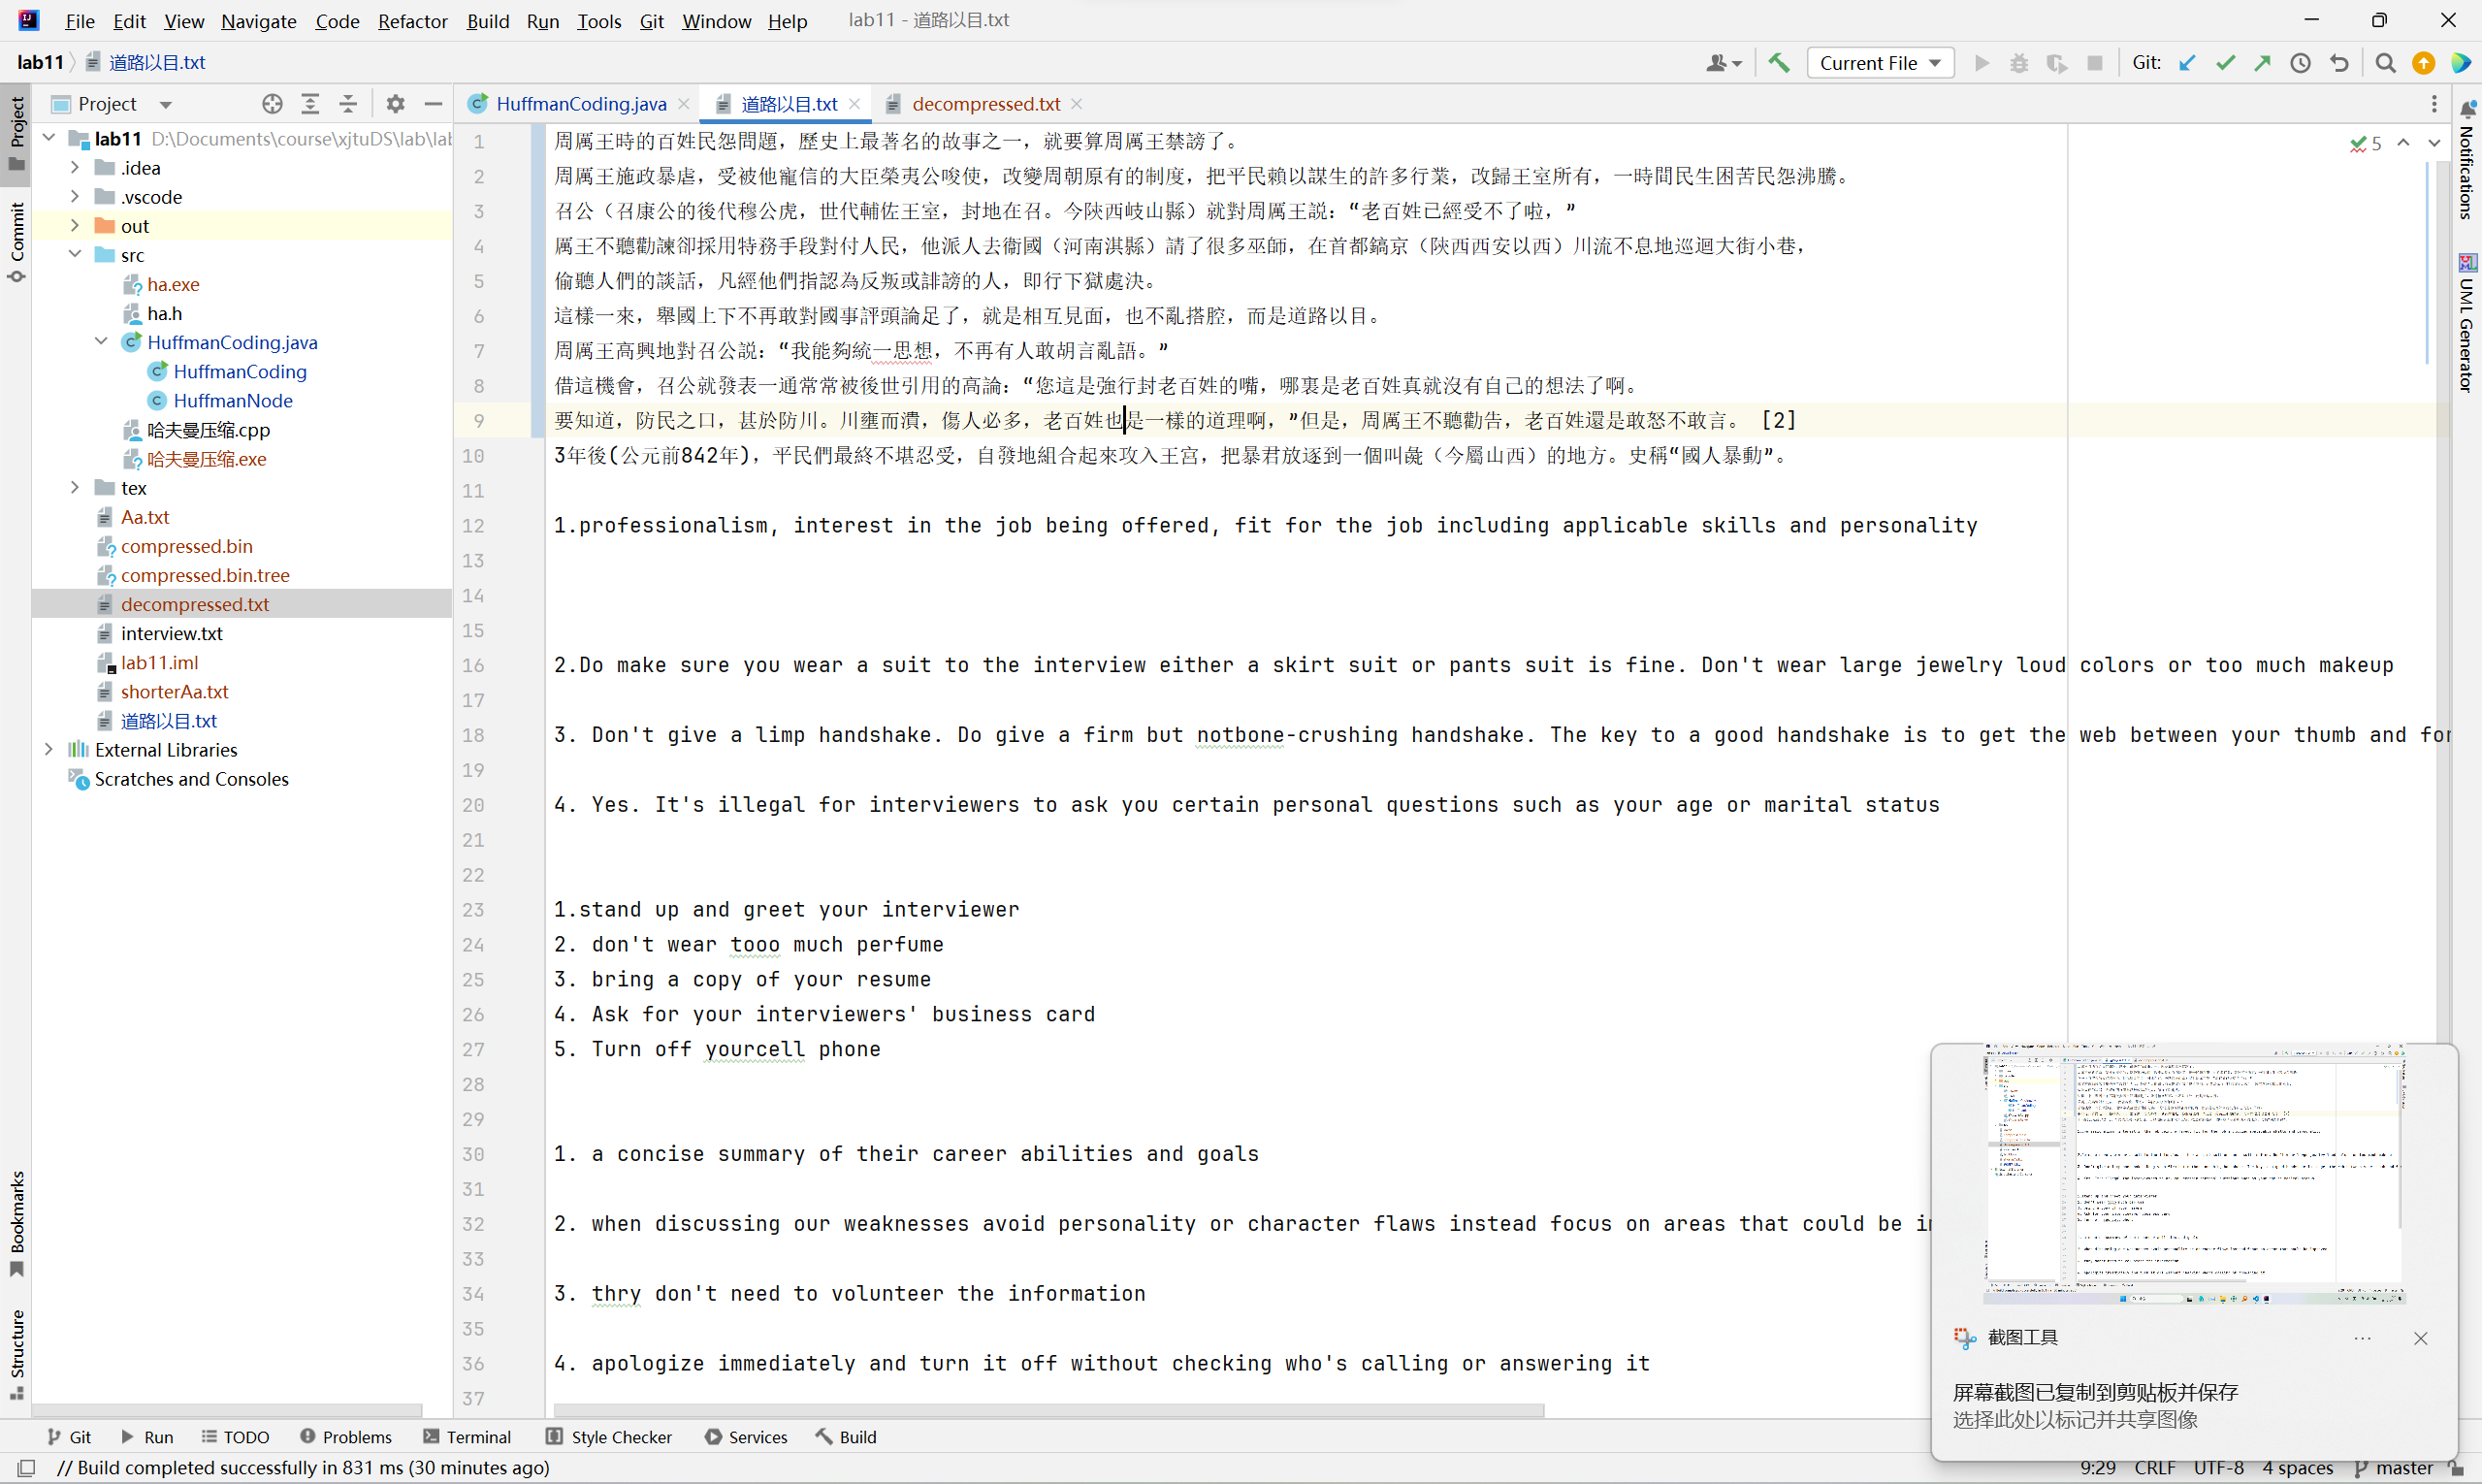
\includegraphics[width=0.9\textwidth]{input.png} % 图片的宽度占正文宽度的50%
  \caption{Input}
  \label{fig:Input}
\end{figure}


\begin{figure}[htbp] 
    \centering
    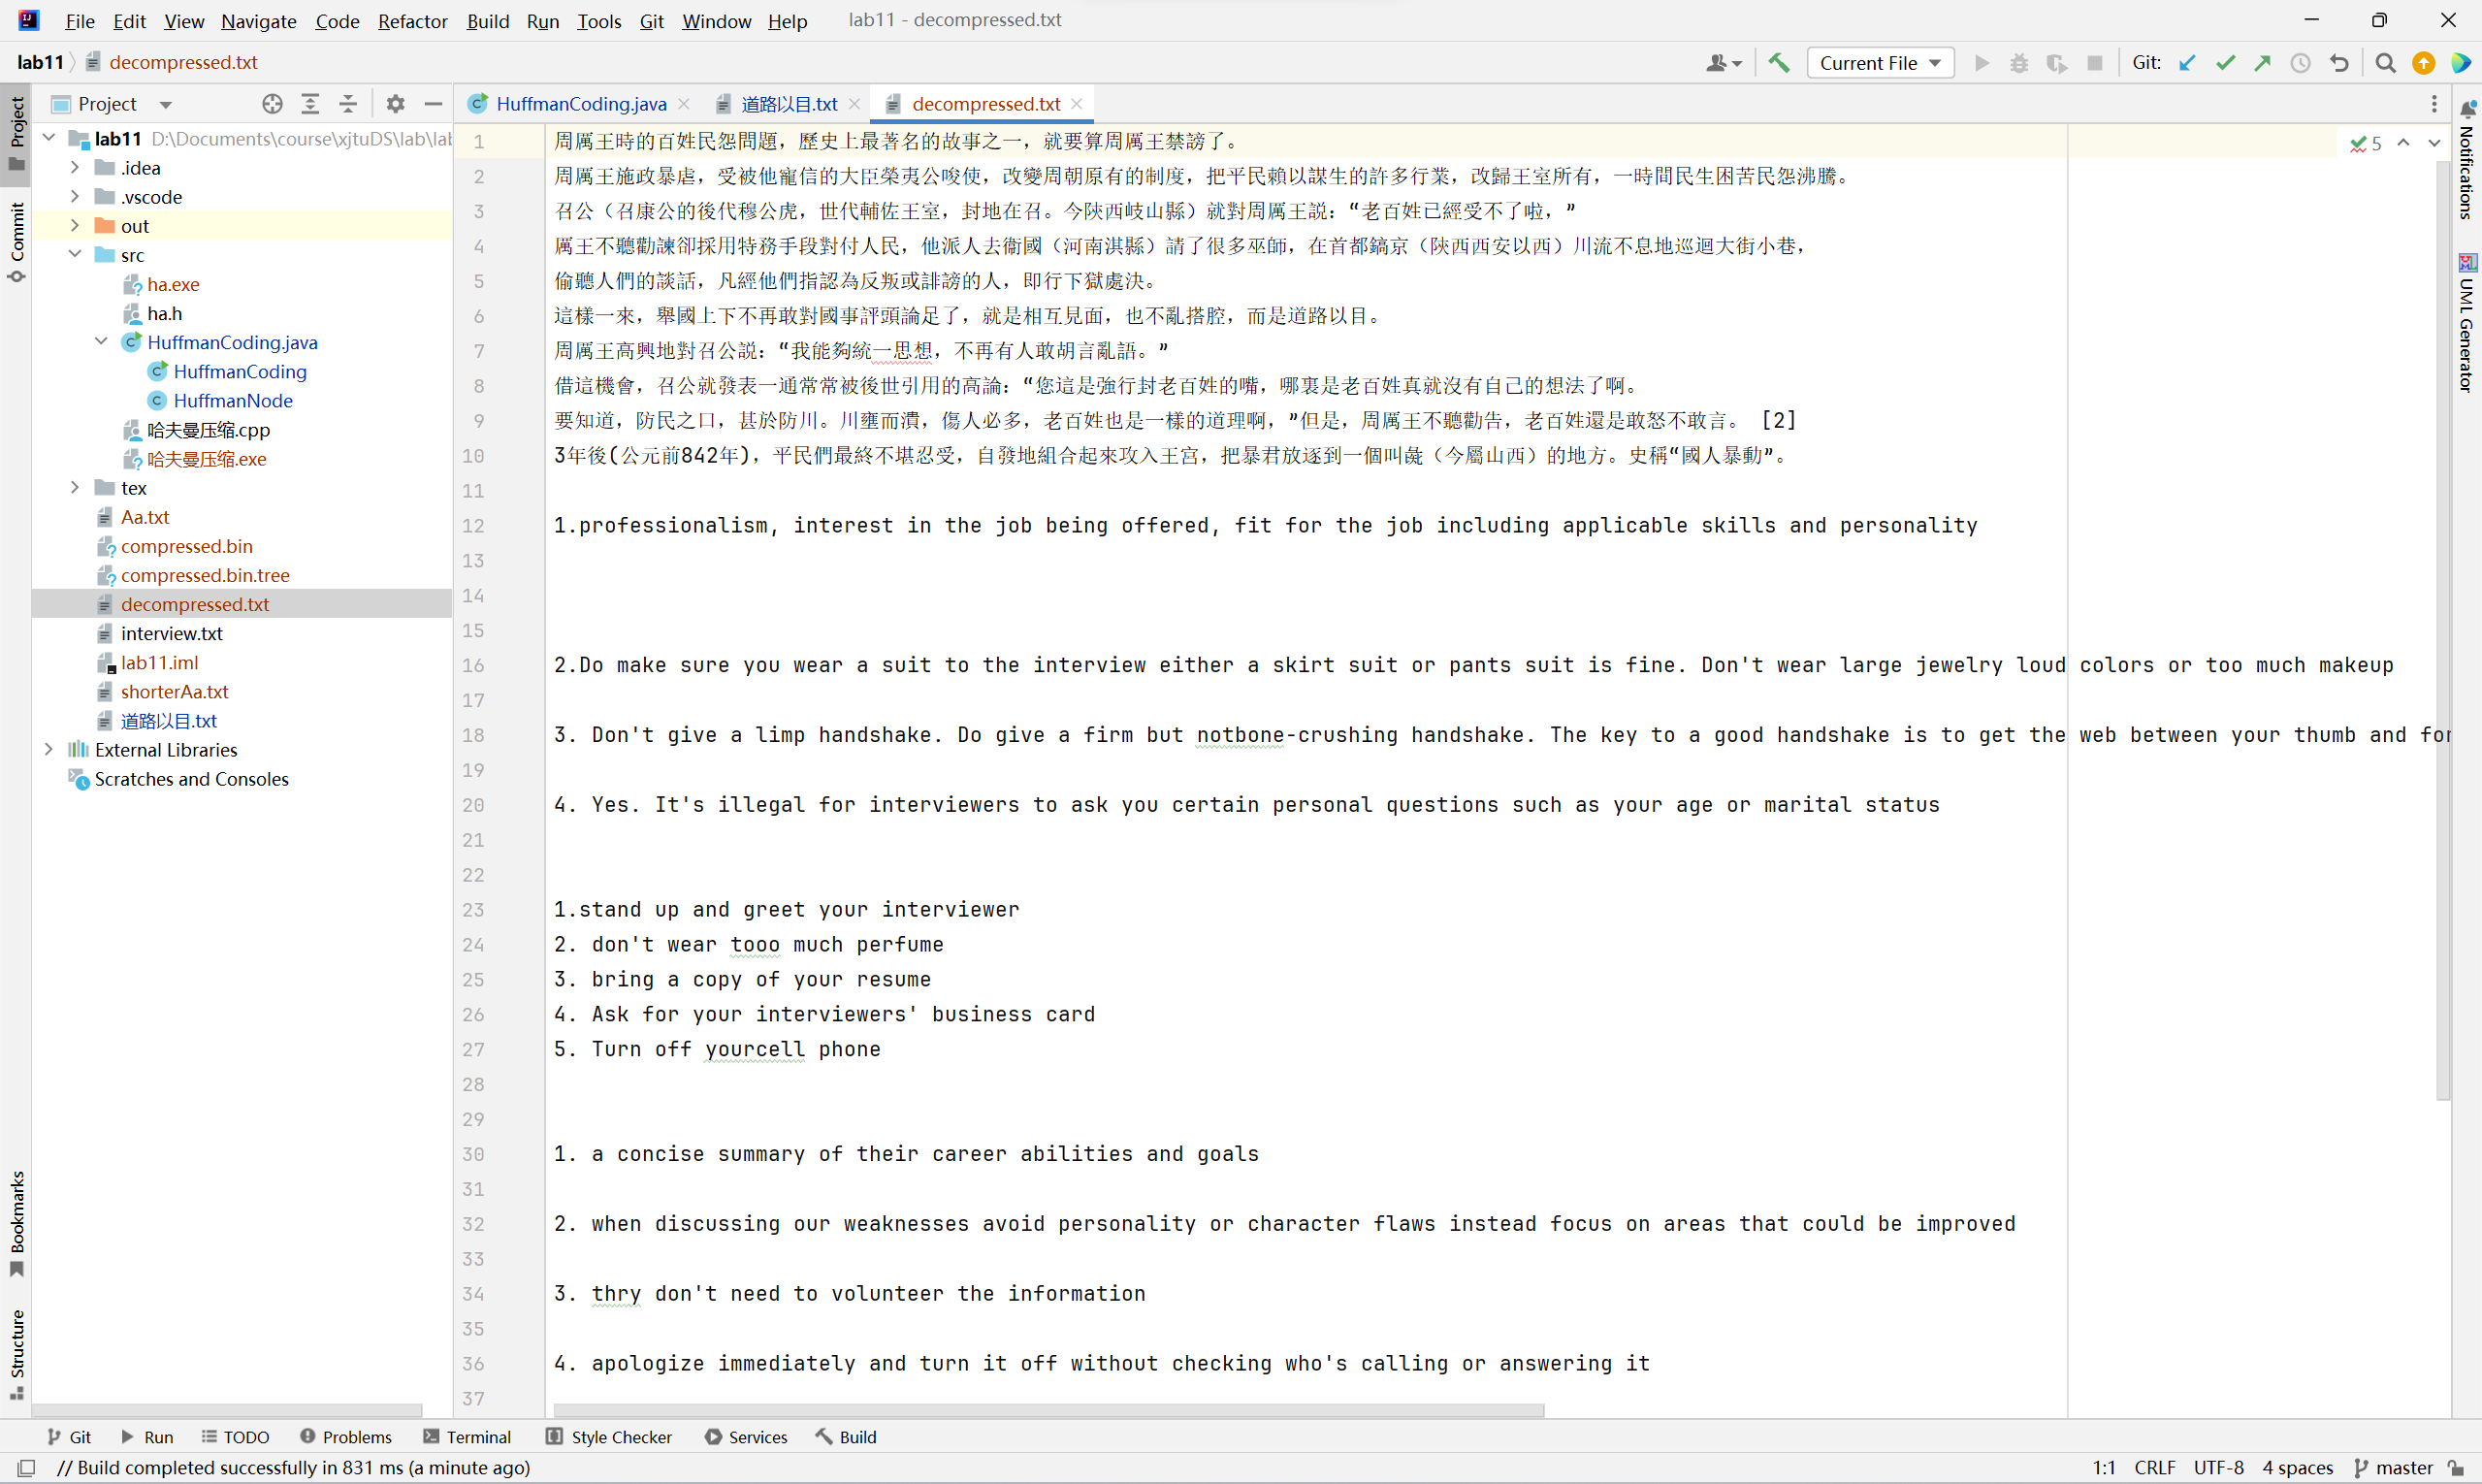
\includegraphics[width=0.9\textwidth]{output.png} % 图片的宽度占正文宽度的50%
    \caption{Output}
    \label{fig:Output}
\end{figure}

\subsection*{时间空间复杂度}

$n$ 是字符的种类数,$m$ 是文件中的字符总数,

\begin{center}
    \begin{tabular}{|l|r|r|} \hline
        Method & Time & Space \\\hline
        \textbf{readFile} & $O(n \log n)$ &  $O(n)$  \\
        \textbf{generateHuffmanCodes} & $O(n)$ & $O(n)$ \\
        \textbf{compressFile} & $O(m)$ & $O(1)$ \\ 
        \textbf{decompressFile} & $O(m)$ & $O(1)$ \\\hline
    \end{tabular}
\end{center}

\textbf{时间复杂度分析:}

1 \textbf{构建哈夫曼树:} $O(n \log n)$ - $n$ 是字符的种类数,构建优先队列的时间复杂度为 $O(n \log n)$。

2 \textbf{生成哈夫曼编码:} $O(n)$ - 递归遍历哈夫曼树,对每个叶子节点生成编码。

3 \textbf{压缩文件:} $O(m)$ - 遍历文件一次。

4 \textbf{解压文件:} $O(m)$ - 遍历压缩文件一次。

\textbf{空间复杂度分析:}

1 \textbf{构建哈夫曼树:} $O(n)$ - 存储字符频率和哈夫曼树节点。

2 \textbf{生成哈夫曼编码:} $O(n)$ - 递归调用时的栈空间。

3 \textbf{压缩文件:} $O(1)$ - 除了原文件和压缩文件外,主要占用空间的是哈夫曼树结构。

4 \textbf{解压文件:} $O(1)$ - 除了压缩文件和解压文件外,主要占用空间的是哈夫曼树结构。


\subsection*{优化分析}

1. \textbf{文件分块压缩:} 对于大文件,可以分块压缩,减少内存占用。

2. \textbf{多线程处理:} 在压缩和解压的过程中,可以使用多线程提高处理速度。

3. \textbf{自适应编码:} 使用自适应编码,动态更新字符频率,适应文件内容的变化。

\newpage
\section*{lab13. 迷宫}
\subsection*{题目}
\begin{abstract}
    %Abstract goes here...
    \textbf{1、问题描述:}

        迷宫实验是取自心理学的一个古典实验。
        在该实验中,把一只老鼠从一个无顶大盒子的门放入,在盒中设置了许多墙,对行进方向形成了多处阻挡。
        盒子仅有一个出口,在出口处放置一块奶酪,吸引老鼠在迷宫中寻找道路以到达出口。
        对同一只老鼠重复进行上述实验,一直到老鼠从入口到出口,而不走错一步。
        老鼠经多次试验终于得到它学习走迷宫的路线。

    \textbf{2、设计功能要求:}

        迷宫由m行n列的二维数组设置,0表示无障碍,1表示有障碍。
        设入口为(1,1),出口为(m,n),每次只能从一个无障碍单元移到周围四个方向上任一无障碍单元。
        编程实现对任意设定的迷宫,求出一条从入口到出口的通路,或得出没有通路的结论。 

        算法输入:代表迷宫入口的坐标

        算法输出:穿过迷宫的结果。 

        算法要点:创建迷宫,试探法查找路。


\end{abstract}



\subsection*{算法思想}

\textbf{解题思想:}

通过深度优先搜索(DFS)解决。
主要思路是从起点开始,按照上、下、左、右的顺序尝试移动,每次移动都标记当前位置,直到找到通路或者无法再移动。如果找到通路,则标记为成功路径,否则标记为死胡同。

\textbf{算法步骤:}
\begin{itemize}
    \item 从入口开始,调用\texttt{findWay}函数。
    \item 在\texttt{findWay}函数中,首先检查当前位置是否是终点,如果是则返回\texttt{true}。
    \item 然后检查当前位置是否是阻塞点,如果是则返回\texttt{false}。
    \item 如果当前位置既不是终点也不是阻塞点,将当前位置标记为已经走过(用2表示),然后递归调用\texttt{findWay}函数,依次尝试上、下、左、右四个方向。
    \item 如果在某个方向找到了通路,则将当前位置标记为成功路径(用6表示),并返回\texttt{true}。
    \item 如果在所有方向都没有找到通路,则将当前位置标记为死胡同(用4表示),并返回\texttt{false}。
    \item 在主函数中,如果\texttt{findWay}返回\texttt{true},则输出迷宫解决方案,否则输出"there is no way out!"。
\end{itemize}


\subsection*{输入输出数据集}

\textbf{IO样例}

\begin{exampleframe}
\textbf{Input:}
\begin{verbatim}
    initial Matrix
    ■■■■■■■■■■
    ■         ■■  ☆
    ■■■  ■        ■
    ■■    ■■  ■■■
    ■■  ■■■■■■■
    ■■  ■■■■■■■
    ■            ■ ■
    ■★■■■■      ■
    ■  ■■■■■■■■
    ■■■■■■■■■■
\end{verbatim}
\textbf{Output:}
\begin{verbatim}
    the solution
    ■■■■■■■■■■
    ■    ▲▲▲■■▲☆
    ■■■▲■▲▲▲▲■
    ■■▲▲■■ ■■■
    ■■▲■■■■■■■
    ■■▲■■■■■■■
    ■▲▲        ■  ■
    ■▲■■■■      ■
    ■  ■■■■■■■■
    ■■■■■■■■■■
\end{verbatim}

\end{exampleframe}
\subsection*{时间空间复杂度}

假设迷宫的大小,$m$为行数,$n$为列数。

\begin{center}
    \begin{tabular}{|l|r|r|} \hline
        Method & Time & Space \\\hline
        \textbf{packup} & $O(m \times n)$ & $O(m \times n)$\\ \hline
    \end{tabular}
\end{center}


\textbf{时间复杂度:}

在最坏情况下,需要遍历迷宫的每一个点,时间复杂度为$O(m \times n)$。

\textbf{空间复杂度:}

递归调用时,需要消耗系统调用栈的空间,最大深度取决于迷宫的大小。空间复杂度为$O(m \times n)$。


\subsection*{优化分析}

\textbf{亮点:}

\textbf{迷宫生成器:} 利用随机函数,生成一个给定大小矩阵的迷宫。

\textbf{改进点:}

\textbf{可视化界面:} 通过图形化界面展示迷宫和搜索过程,使得结果更直观。这可以通过引入图形库来实现。


\iffalse
\fi


\end{document}
